\documentclass[12pt]{article}
\usepackage{baseset}
\usepackage{myproblem}
\usepackage{stackengine}
\DeclareSymbolFont{operators}{OT1}{ntxtlf}{m}{n}
\SetSymbolFont{operators}{bold}{OT1}{ntxtlf}{b}{n}
\usepackage{wasysym}
\newcommand{\RomanNumeralCaps}[1]
{\MakeUppercase{\romannumeral #1}}
\usepackage{tabularx}
\usepackage{enumitem}

\begin{document}
\begin{tabularx}{\textwidth}{Xr}
{\Large \textbf{Праки}} & Взлёт $27.11.2023$ \\
\end{tabularx}
\noindent\rule{\textwidth}{0.4pt}
\begin{enumerate}
    \item Вам на отдельном листе дано изображение диска спиральной галактики UGC $11914$ (слева) в фильтре R (поэтому спиральные рукава не видны). Черными сплошными линиями показаны изофоты (линии одинаковой поверхностной яркости). На правом изображении находится диаграмма положение-скорость вдоль большой оси для той же галактики (скорость дана относительно нашей Галактики). Яркость означает количество вещества на данном расстоянии, движущегося с данной лучевой скоростью (чем темнее, тем больше вещества). Положение центра диска обозначено пунктирными линиями.
    \begin{itemize}
        \item Определите угол наклона галактики к картинной плоскости и позиционный угол, соответствующий положению ее большой оси (позиционный угол отсчитывается от направления на север против часовой стрелки).
        \item Оцените расстояние до галактики.
        \item Постройте кривую вращения галактики (зависимость линейной скорости вращения от расстояния до центра).
        \item Оцените массу балджа и массу всей галактики.
        \item Выделите на кривой вращения два участка, связанные с балджем и гало. Пренебрегая плоской компонентой (диском) и предполагая распределение плотности сферически симметричным, определите зависимость плотности от радиуса.
    \end{itemize}
    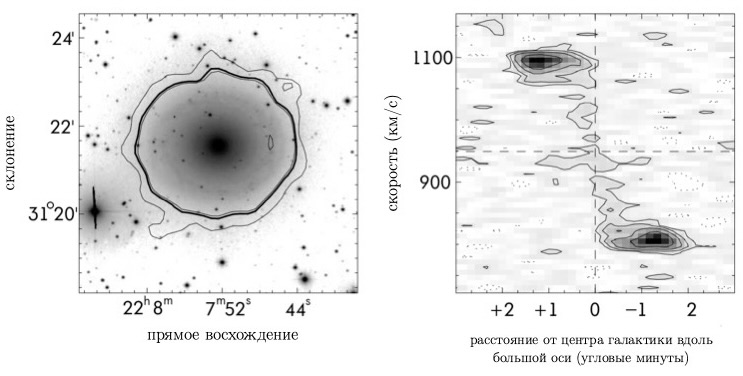
\includegraphics[width = \linewidth]{img5.jpeg}
    \newpage
    \item Вам дана кеограмма (на отдельном листе), полученная астрономом в течение одного года. По вертикальной оси отложены месяцы, по горизонтальной -- гражданское время. Часовой пояс пункта наблюдения UTC+1.
    Определите географические координаты пункта наблюдения. Качественно объясните природу светлых наклонных полос: чем они вызваны и почему они наклонные. Качественно объясните несимметричность темной области относительно вертикальной оси.
    Кеограмма была получена следующим образом. Каждые 15 секунд в течение года неподвижная камера с объективом «рыбий глаз» (fisheye) делала снимок всего неба. Затем узкая полоска вдоль небесного меридиана вырезалась и сужалась до квадратика. Горизонтальная полоска, полученная из таких квадратиков за сутки, составляет одну строку кеограммы. 365 полосок, расположенных вертикально, составляют полное изображение кеограммы.
    Кроме того, вам дан график зависимости освещенности (в люксах) квадратного приемника в зависимости от зенитного расстояния Солнца в ясную погоду. Чувствительность камеры, использованной для создания кеограммы, резко падает при освещенности менее чем 0.03 лк.

    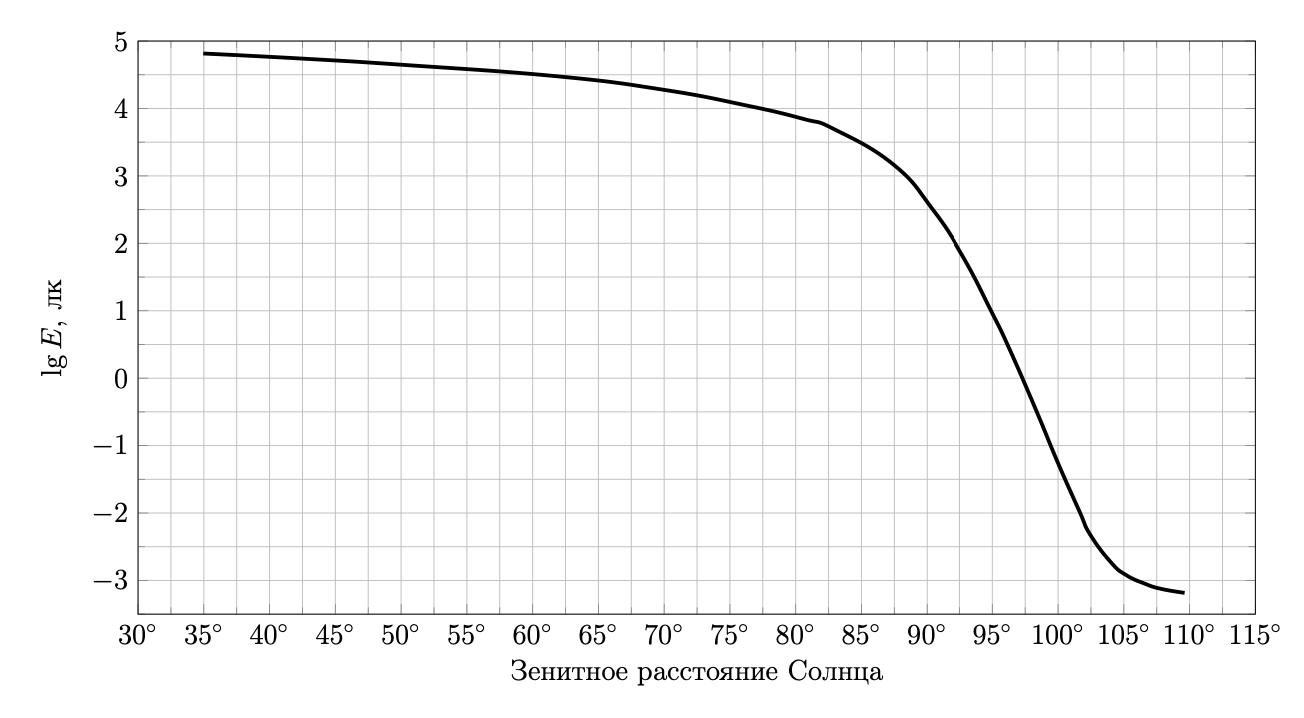
\includegraphics[width = 0.9\linewidth]{img1.png}

    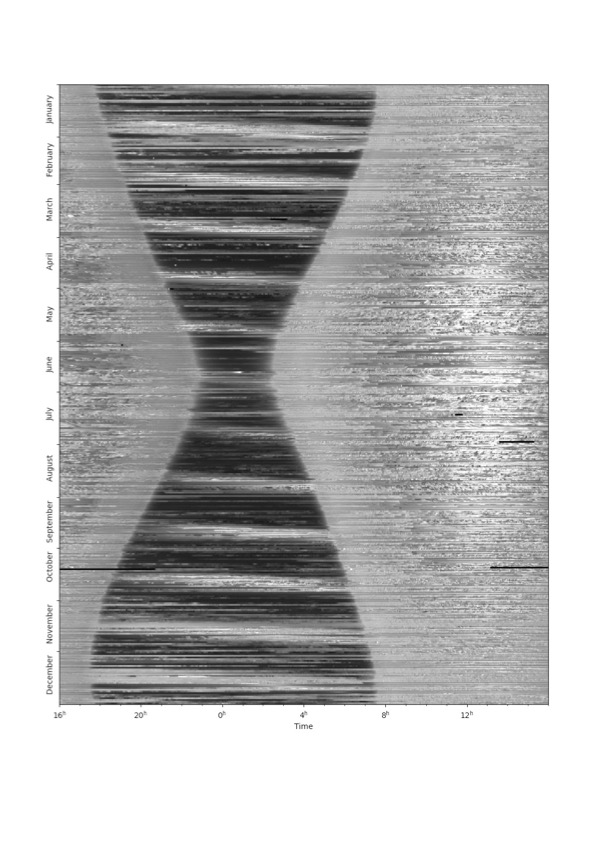
\includegraphics[width = \linewidth]{img6.jpg}
    \newpage
    \item Вам дан коллаж фотографий затмения, произошедшего 4 декабря. Определите высоту Солнца над горизонтом в момент максимальной фазы затмения, широту места наблюдения, расстояние до людей на крыше здания от места съемки. Определите, куда движется Солнце относительно наблюдателя (влево или вправо) и куда движется Луна относительно Солнца. Найдите время, через которое делались кадры для коллажа. Можно считать, что нижняя граница изображения параллельна математическому горизонту.
    \begin{center}
        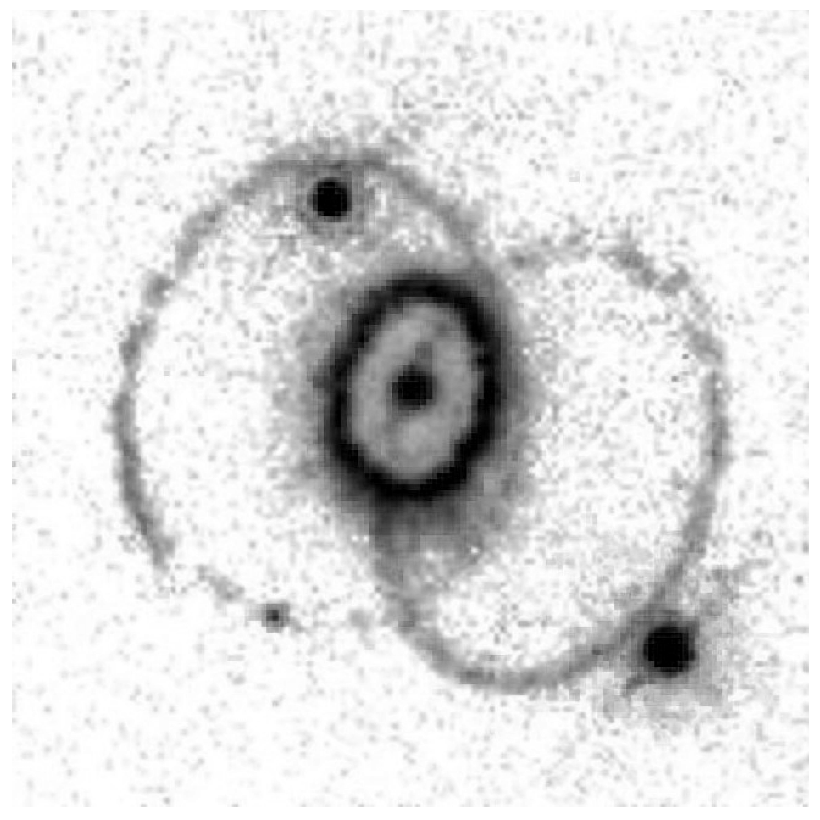
\includegraphics[width = 0.7\linewidth]{img3.png}
    \end{center}
    \item Вам дано негативное изображение, полученное при наблюдении остатка вспышки сверхновой с высоким разрешением. Две кольцеобразных структуры -- это два параллельных кольца одинакового радиуса, расположенных симметрично по отношению к сверхновой и состоящих из вещества, выброшенного предшественником сверхновой, и подсвеченного во время вспышки.
    \item Вам дано изображение (негатив) корональной петли, образовавшейся на видимом краю диска Солнца из-за выхода силовых линий магнитного поля. Оцените объем этой корональной петли, считая ее изогнутой трубкой.
    
    \newpage
    
    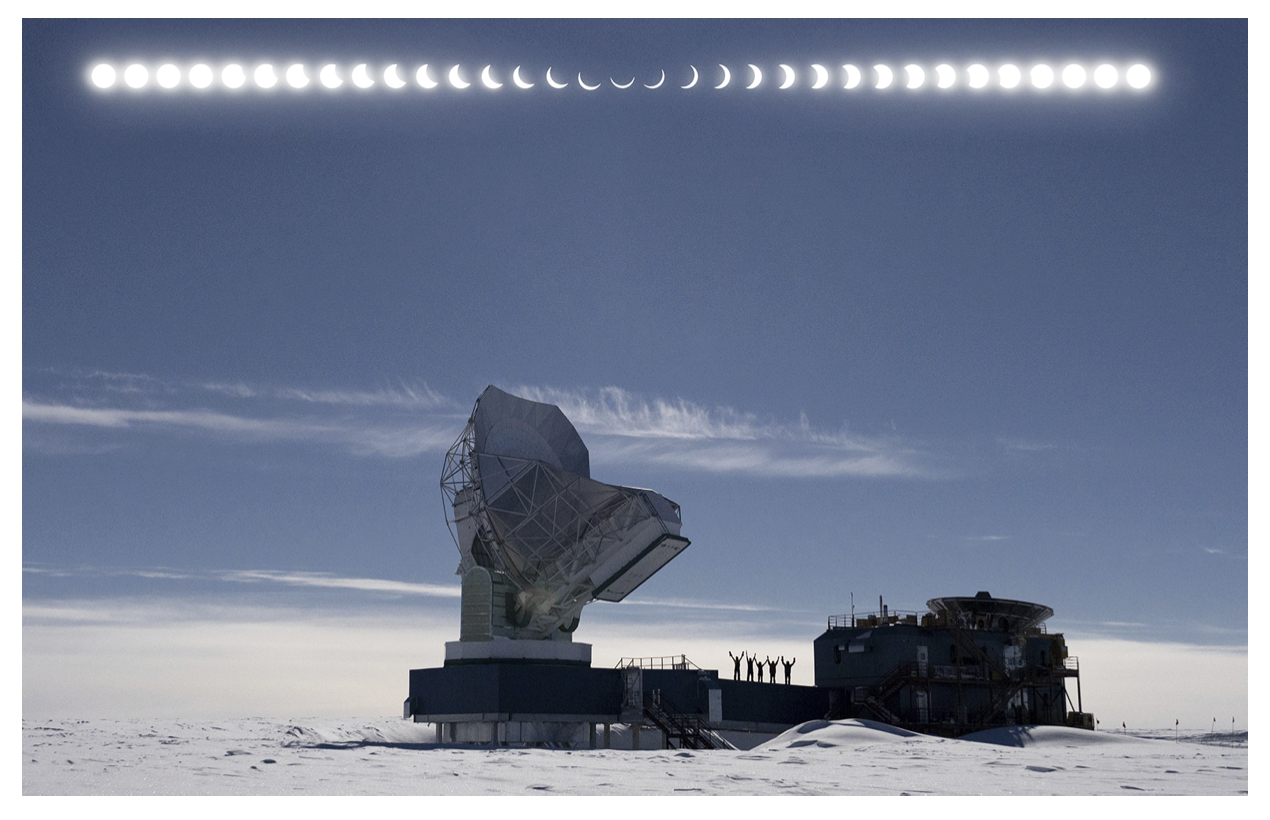
\includegraphics[width = \linewidth]{img2.png}
    
    
    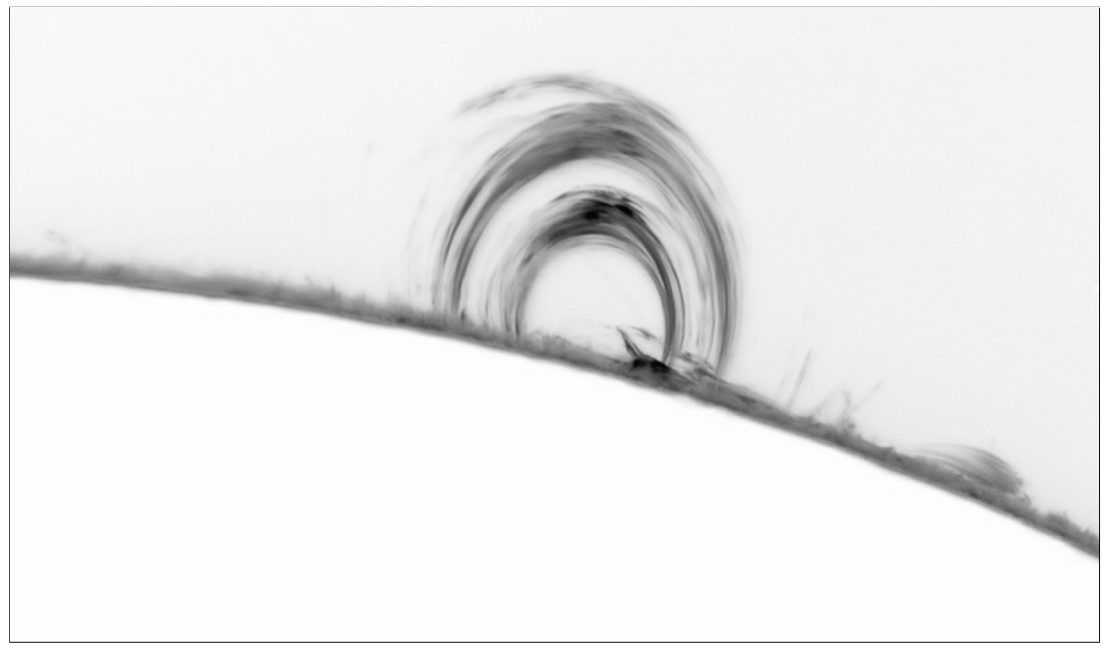
\includegraphics[width = \linewidth]{img4.png}

\end{enumerate}
\end{document}